\documentclass{article}

%\usepackage[math,lf,footnotefigures]{MyriadPro}
\renewcommand\familydefault{\sfdefault} 
\usepackage[T1]{fontenc}

\usepackage{tikz}
\usetikzlibrary{arrows}
\usetikzlibrary{arrows.meta}
\usetikzlibrary{positioning}

\usepackage{xcolor}
\definecolor{ufzgray1}{RGB}{81,81,81}
\definecolor{ufzgray2}{RGB}{156,156,156}
\definecolor{ufzgray3}{RGB}{185,185,185}
\definecolor{ufzgray4}{RGB}{230,230,230}

\begin{document}
	
\pagestyle{empty}

\hspace*{-3cm}
	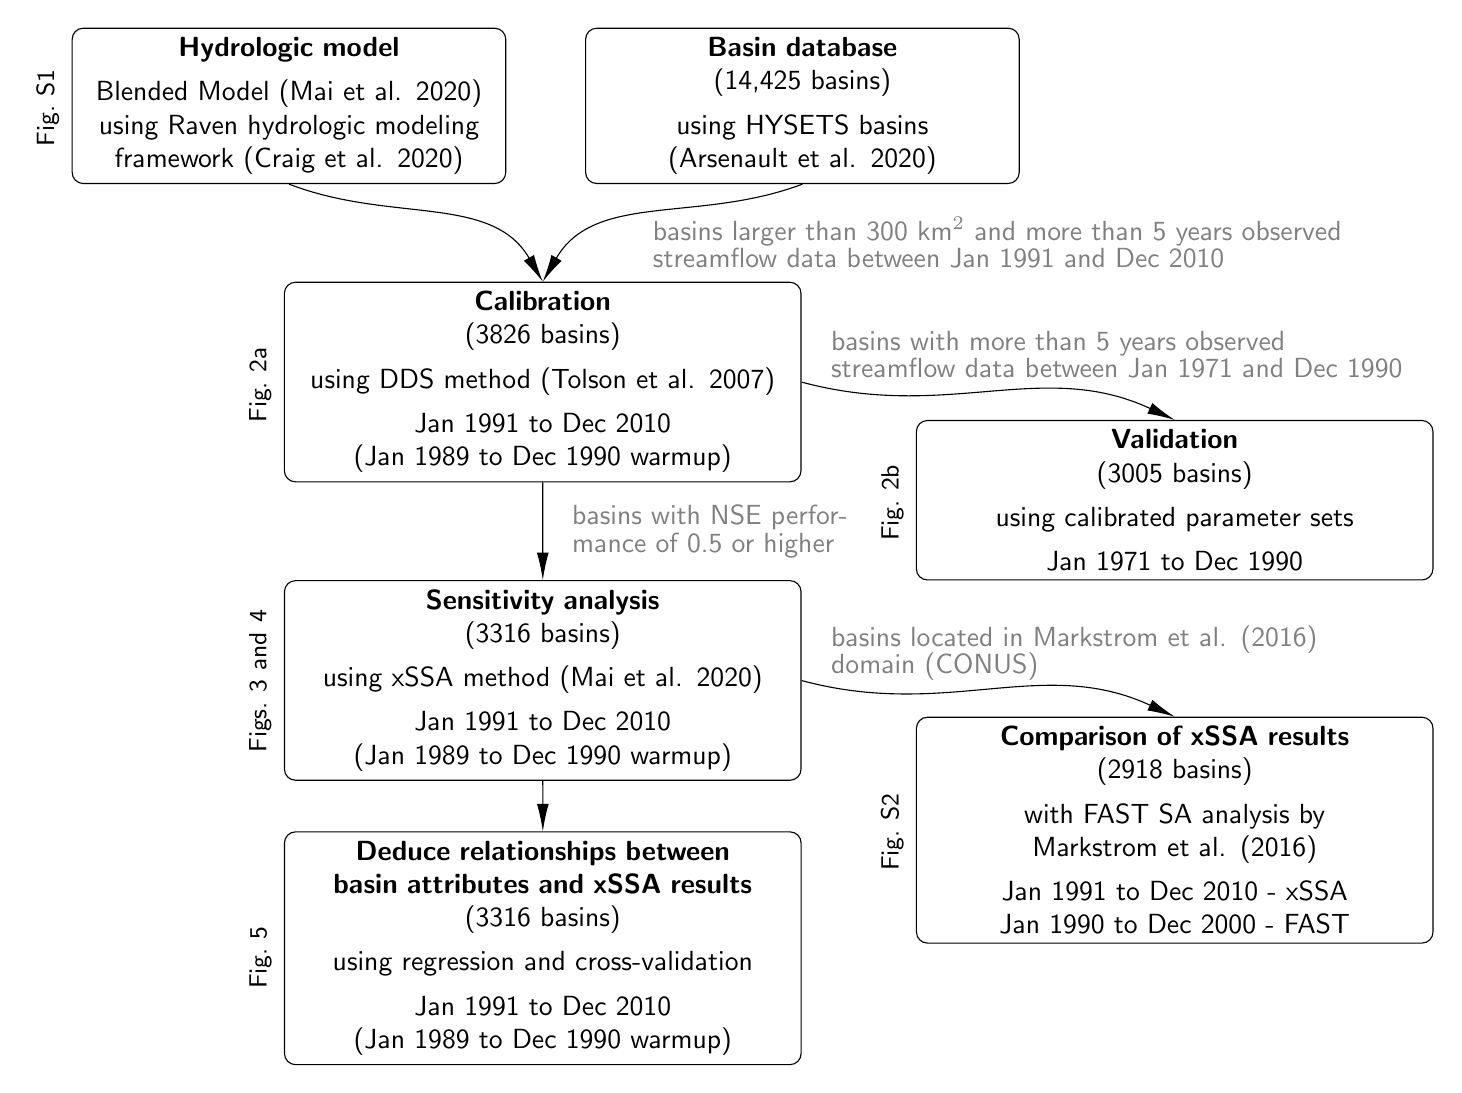
\begin{tikzpicture}[scale=2.5]
		\tikzstyle{block} = [rectangle, draw, fill=white!20, 
		text width=18em, text centered, rounded corners, minimum height=1em]
		\tikzstyle{noblock} = [rectangle, fill=white!20, 
		text width=18em, rounded corners, minimum height=1em]
		\tikzstyle{abcblock} = [rectangle, fill=white!20, 
		text width=1em, rounded corners, minimum height=1em]
		\tikzstyle{line} = [draw, -latex']
		\tikzstyle{line} = [draw,latex'-latex'new]
		
		% Model
		\node [block, node distance=2.5cm, text width=15em] (a1a) {\textbf{Hydrologic model}\\[4pt] Blended Model (Mai et al. 2020)\\ using Raven hydrologic modeling\\ framework (Craig et al. 2020)};
		\node [noblock,rotate=90,align=center,left=0.3cm of a1a.west,text width=0.4em,xshift=-0.25cm] (a1asec) {\small Fig.~S1\\};
		
		% Basin database
		\node [block, node distance=2.5cm, text width=15em, right=1.0cm of a1a.east] (a1b) {\textbf{Basin database}\\(14,425 basins)\\[4pt] using HYSETS basins (Arsenault et al. 2020)};
		
		% Calibration
		\node [block, below=1.24cm of a1b.south, node distance=2.5cm, xshift=-3.3cm] (a2) {\textbf{Calibration}\\(3826 basins)\\[4pt] using DDS method (Tolson et al. 2007)\\[4pt]Jan 1991 to Dec 2010\\(Jan 1989 to Dec 1990 warmup)};
		\node [noblock,rotate=90,align=center,left=0.3cm of a2.west,text width=0.4em,xshift=-0.25cm] (a2sec) {\small Fig.~2a\\};
		
		% Validation
		\node [block, right=1.45cm of a2.east, node distance=2.5cm,yshift=-1.5cm] (a3) {\textbf{Validation}\\(3005 basins)\\[4pt]using calibrated parameter sets\\[4pt] Jan 1971 to Dec 1990};
		\node [noblock,rotate=90,align=center,left=0.3cm of a3.west,text width=0.4em,xshift=-0.25cm] (a3sec) {\small Fig.~2b\\};
		
		% SA
		\node [block, below=1.24cm of a2.south, node distance=2.5cm] (a4) {\textbf{Sensitivity analysis}\\(3316 basins)\\[4pt] using xSSA method (Mai et al. 2020)\\[4pt] Jan 1991 to Dec 2010\\(Jan 1989 to Dec 1990 warmup)};
		\node [noblock,rotate=90,align=center,left=0.3cm of a4.west,text width=0.4em,xshift=-0.65cm] (a4sec) {\small Figs.~3~and~4\\};
		
		% Comparison
		\node [block, right=1.45cm of a4.east, node distance=2.5cm,yshift=-1.9cm] (a6) {\textbf{Comparison of xSSA results}\\(2918 basins)\\[4pt] with FAST SA analysis by\\ Markstrom et al. (2016)\\[4pt] Jan 1991 to Dec 2010 - xSSA\\ Jan 1990 to Dec 2000 - FAST};
		\node [noblock,rotate=90,align=center,left=0.3cm of a6.west,text width=0.4em,xshift=-0.25cm] (a6sec) {\small Fig.~S2\\};
		
		% Functional relationships
		\node [block, below=0.64cm of a4.south, node distance=2.5cm] (a5) {\textbf{Deduce relationships between}\\\textbf{basin attributes and xSSA results}\\ (3316 basins)\\[4pt] using regression and cross-validation\\[4pt] Jan 1991 to Dec 2010\\(Jan 1989 to Dec 1990 warmup)};
		\node [noblock,rotate=90,align=center,left=0.3cm of a5.west,text width=0.4em,xshift=-0.25cm] (a5sec) {\small Fig.~5\\};

		% arrows
		\draw [-{Latex[length=3.5mm, width=1.5mm]}] (a1a.south) to[out=0,in=120,yshift=-0.2cm] (a2.north);
		
		\draw [-{Latex[length=3.5mm, width=1.5mm]}] (a1b.south) to[out=180,in=60,yshift=-0.2cm] (a2.north);
		\node [below=0.5cm of a1b.south, node distance=2.5cm,xshift=2.55cm,yshift=0.20cm,text width=8.9cm,color=gray] {basins larger than 300~km$^\mathrm{2}$ and more than 5 years observed\\[-2pt] streamflow data between Jan 1991 and Dec 2010};
		%
		\draw [-{Latex[length=3.5mm, width=1.5mm]},yshift=-0.2cm] (a2.east) to[out=0,in=155,yshift=-0.2cm] (a3.north);
		\node [right=0.25cm of a2.east, node distance=2.5cm,yshift=0.35cm,text width=7.5cm,color=gray] {basins with more than 5 years observed\\[-2pt] streamflow data between Jan 1971 and Dec 1990};
		%
		\draw [-{Latex[length=3.5mm, width=1.5mm]}] (a4.east) to[out=0,in=155,yshift=-0.2cm] (a6.north);
		\node [right=0.25cm of a4.east, node distance=2.5cm,yshift=0.35cm,text width=7.0cm,color=gray] {basins located in Markstrom et al. (2016)\\[-2pt] domain (CONUS)};
		%
		\draw [-{Latex[length=3.5mm, width=1.5mm]}] (a2.south) -- (a4.north)node [pos=0.5, align=left,right,text width=6cm,xshift=0.25cm,color=gray] {basins with NSE perfor-\\[-2pt] mance of 0.5 or higher};
		\draw [-{Latex[length=3.5mm, width=1.5mm]}] (a4.south) -- (a5.north);
		
	\end{tikzpicture}
	
	
%	\hspace*{-3cm}
%	\begin{tikzpicture}[scale=2.5]
%	\tikzstyle{block} = [rectangle, draw, fill=white!20, 
%	text width=1em, text centered, rounded corners, minimum height=1em]
%	\tikzstyle{noblock} = [rectangle, fill=white!20, 
%	text width=12em, rounded corners, minimum height=1em]
%	\tikzstyle{line} = [draw, -latex']
%	
%	% process names
%	\node [noblock,align=left] (A) {Process 1\\ (e.g., infiltration)};
%	\node [noblock,align=left,below of=A] (B) {Process 2\\ (e.g., quickflow)};
%	\node [noblock,align=left,below of=B] (C) {Process 3\\ (e.g., evaporation)};
%	\node [noblock,align=left,below of=C] (D) {Process 4\\ (e.g., baseflow)};
%	\node [noblock,align=left,below of=D] (E) {Process 5\\ (e.g., snow balance)};
%	\node [noblock,align=left,below of=E] (F) {Process 6\\ (e.g., surf. runoff convol.)};
%	\node [noblock,align=left,below of=F] (G) {Process 7\\ (e.g., delay. runoff convol.)};
%	\node [noblock,align=left,below of=G] (H) {Process 8\\ (e.g., potential melt)};
%	\node [noblock,align=left,below of=H] (I) {Process 9\\ (e.g., percolation)};
%	\node [noblock,align=left,below of=I] (J) {Process 10\\ (e.g., remainder)};
%	%\node [noblock,align=left,below of=J] (K) {Process 11\\ (e.g., remainder)};
%	
%	% process options (simple setup)
%	\node [block, node distance=1.5cm,right of=A, xshift=0.7cm] (a1) {$A_1$};
%	\node [block, node distance=1.5cm,right of=a1] (a2) {$A_2$};
%	\node [block, node distance=1.5cm,right of=B] (b1) {$B_1$};
%	\node [block, node distance=1.5cm,right of=b1] (b2) {$B_2$};
%	\node [block, node distance=1.5cm,right of=b2] (b3) {$B_3$};
%	\node [block, node distance=1.5cm,right of=C, xshift=0.7cm] (c1) {$C_1$};
%	\node [block, node distance=1.5cm,right of=c1] (c2) {$C_2$};
%	
%	% process options (realistic setup)
%	\node [block, node distance=1.5cm,right of=a2, xshift=2.1cm] (d1) {$D_1$};
%	\node [block, node distance=1.5cm,right of=d1] (d2) {$D_2$};
%	\node [block, node distance=1.5cm,right of=b3, xshift=0.5cm] (e1) {$E_1$};
%	\node [block, node distance=1.5cm,right of=e1] (e2) {$E_2$};
%	\node [block, node distance=1.5cm,right of=e2] (e3) {$E_3$};
%	\node [block, node distance=1.5cm,right of=c2, xshift=2.1cm] (f1) {$F_1$};
%	\node [block, node distance=1.5cm,right of=f1] (f2) {$F_2$};
%	
%	% process options (Raven setup)
%	\node [block, node distance=1.5cm,right of=d2, xshift=1.2cm] (m1) {$M_1$};
%	\node [block, node distance=1.5cm,right of=m1] (m2) {$M_2$};
%	\node [block, node distance=1.5cm,right of=m2] (m3) {$M_3$};
%	\node [block, node distance=1.5cm,right of=e3, xshift=0.5cm] (n1) {$N_1$};
%	\node [block, node distance=1.5cm,right of=n1] (n2) {$N_2$};
%	\node [block, node distance=1.5cm,right of=n2] (n3) {$N_3$};
%	\node [block, node distance=1.5cm,right of=f2, xshift=2.0cm] (o1) {$O_1$};
%	\node [block, node distance=1.5cm,right of=o1] (o2) {$O_2$};
%	\node [block, node distance=1.5cm,right of=D, xshift=10.8cm] (p1) {$P_1$};
%	\node [block, node distance=1.5cm,right of=p1] (p2) {$P_2$};
%	\node [block, node distance=1.5cm,right of=E, xshift=10.0cm] (q1) {$Q_1$};
%	\node [block, node distance=1.5cm,right of=q1] (q2) {$Q_2$};
%	\node [block, node distance=1.5cm,right of=q2] (q3) {$Q_3$};
%	%\node [block, node distance=1.5cm,right of=q3] (q4) {$Q_4$};
%	\node [block, node distance=1.5cm,right of=F, xshift=11.5cm] (r1) {$R_1$};
%	\node [block, node distance=1.5cm,right of=G, xshift=11.5cm] (s1) {$S_1$};
%	\node [block, node distance=1.5cm,right of=H, xshift=11.5cm] (t1) {$T_1$};
%	\node [block, node distance=1.5cm,right of=I, xshift=11.5cm] (u1) {$U_1$};
%	\node [block, node distance=1.5cm,right of=J, xshift=11.5cm] (v1) {$V_1$};
%	%\node [block, node distance=1.5cm,right of=K, xshift=11.5cm] (w1) {$W_1$};
%	
%	% parameters (simple setup)
%	\node [align=left, right of=a1, xshift=-0.4cm] {\footnotesize $x_1$};
%	\node [align=left, right of=a2, xshift=-0.4cm] {\footnotesize $-$};
%	\node [align=left, right of=b1, xshift=-0.4cm] {\footnotesize $x_2$};
%	\node [align=left, right of=b2, xshift=-0.4cm] {\footnotesize $x_3$};
%	\node [align=left, right of=b3, xshift=-0.4cm] {\footnotesize $x_4$\\[-4pt]\footnotesize $x_5$};
%	\node [align=left, right of=c1, xshift=-0.4cm] {\footnotesize $x_6$};
%	\node [align=left, right of=c2, xshift=-0.4cm] {\footnotesize $x_7$};
%	
%	% parameters (realistic setup)
%	\node [align=left, right of=d1, xshift=-0.4cm] {\footnotesize $x_1$};
%	\node [align=left, right of=d2, xshift=-0.4cm] {\footnotesize $x_1$\\[-4pt]\footnotesize $x_2$};
%	\node [align=left, right of=e1, xshift=-0.4cm] {\footnotesize $x_2$};
%	\node [align=left, right of=e2, xshift=-0.4cm] {\footnotesize $x_3$};
%	\node [align=left, right of=e3, xshift=-0.4cm] {\footnotesize $x_4$\\[-4pt]\footnotesize $x_5$};
%	\node [align=left, right of=f1, xshift=-0.4cm] {\footnotesize $x_6$};
%	\node [align=left, right of=f2, xshift=-0.4cm] {\footnotesize $x_3$\\[-4pt]\footnotesize $x_7$};
%	
%	% parameters (Raven setup)
%	\node [align=left, right of=m1, xshift=-0.4cm] {\footnotesize $x_{1}$\\[-4pt]\footnotesize $x_{29}$};
%	\node [align=left, right of=m2, xshift=-0.4cm] {\footnotesize $x_{2}$\\[-4pt]\footnotesize $x_{29}$};
%	\node [align=left, right of=m3, xshift=-0.4cm] {\footnotesize $x_{3}$\\[-4pt]\footnotesize $x_{29}$};
%	\node [align=left, right of=n1, xshift=-0.4cm] {\footnotesize $x_{4}$\\[-4pt]\footnotesize $x_{29}$};
%	\node [align=left, right of=n2, xshift=-0.4cm] {\footnotesize $x_{5}$\\[-4pt]\footnotesize $x_{6}$\\[-4pt]\footnotesize $x_{29}$};
%	\node [align=left, right of=n3, xshift=-0.4cm] {\footnotesize $x_{5}$\\[-4pt]\footnotesize $x_{6}$\\[-4pt]\footnotesize $x_{7}$\\[-4pt]\footnotesize $x_{29}$};
%	\node [align=left, right of=o1, xshift=-0.4cm] {\footnotesize $x_{8}$\\[-4pt]\footnotesize $x_{29}$};
%	\node [align=left, right of=o2, xshift=-0.4cm] {\footnotesize $x_{8}$\\[-4pt]\footnotesize $x_{9}$\\[-4pt]\footnotesize $x_{10}$\\[-4pt]\footnotesize $x_{29}$};
%	\node [align=left, right of=p1, xshift=-0.4cm] {\footnotesize $x_{11}$};
%	\node [align=left, right of=p2, xshift=-0.4cm] {\footnotesize $x_{11}$\\[-4pt]\footnotesize $x_{12}$};
%	
%	\node [align=left, right of=q1, xshift=-0.4cm] {\footnotesize $x_{13}$\\[-8pt]\footnotesize $\ldots$\\[-6pt]\footnotesize $x_{18}$};
%	\node [align=left, right of=q2, xshift=-0.4cm] {\footnotesize $-$};
%	\node [align=left, right of=q3, xshift=-0.4cm] {\footnotesize $x_{18}$\\[-4pt]\footnotesize $x_{19}$};
%	%\node [align=left, right of=q4, xshift=-0.4cm] {\footnotesize $x_{18}$\\[-4pt]\footnotesize $x_{19}$\\[-4pt]\footnotesize $x_{20}$};
%	
%	\node [align=left, right of=r1, xshift=-0.4cm] {\footnotesize $x_{20}$\\[-4pt]\footnotesize $x_{21}$};
%	
%	\node [align=left, right of=s1, xshift=-0.4cm] {\footnotesize $x_{22}$\\[-4pt]\footnotesize $x_{23}$};
%	
%	\node [align=left, right of=t1, xshift=-0.4cm] {\footnotesize $x_{24}$\\[-8pt]\footnotesize $\ldots$\\[-6pt]\footnotesize $x_{27}$};
%	
%	\node [align=left, right of=u1, xshift=-0.4cm] {\footnotesize $x_{28}$\\[-4pt]\footnotesize $x_{29}$\\[-4pt]\footnotesize $x_{30}$};
%	
%	%\node [align=left, right of=v1, xshift=-0.4cm] {\footnotesize $x_{30}$\\[-4pt]\footnotesize $x_{31}$};
%	
%	\node [align=left, right of=v1, xshift=-0.4cm] {\footnotesize $-$};
%	
%	% lines A-B (simple setup)
%	\draw (a1.south) -- (b1.north);
%	\draw (a1.south) -- (b2.north);
%	\draw (a1.south) -- (b3.north);
%	\draw (a2.south) -- (b1.north);
%	\draw (a2.south) -- (b2.north);
%	\draw (a2.south) -- (b3.north);
%	
%	% lines B-C (simple setup)
%	\draw (b1.south) -- (c1.north);
%	\draw (b1.south) -- (c2.north);
%	\draw (b2.south) -- (c1.north);
%	\draw (b2.south) -- (c2.north);
%	\draw (b3.south) -- (c1.north);
%	\draw (b3.south) -- (c2.north);
%	
%	% lines A-B (realistic setup)
%	\draw (d1.south) -- (e1.north);
%	\draw (d1.south) -- (e2.north);
%	\draw (d1.south) -- (e3.north);
%	\draw (d2.south) -- (e1.north);
%	\draw (d2.south) -- (e2.north);
%	\draw (d2.south) -- (e3.north);
%	
%	% lines B-C (realistic setup)
%	\draw (e1.south) -- (f1.north);
%	\draw (e1.south) -- (f2.north);
%	\draw (e2.south) -- (f1.north);
%	\draw (e2.south) -- (f2.north);
%	\draw (e3.south) -- (f1.north);
%	\draw (e3.south) -- (f2.north);
%	
%	% lines M-N (Raven setup)
%	\draw (m1.south) -- (n1.north);
%	\draw (m1.south) -- (n2.north);
%	\draw (m1.south) -- (n3.north);
%	\draw (m2.south) -- (n1.north);
%	\draw (m2.south) -- (n2.north);
%	\draw (m2.south) -- (n3.north);
%	\draw (m3.south) -- (n1.north);
%	\draw (m3.south) -- (n2.north);
%	\draw (m3.south) -- (n3.north);
%	
%	% lines N-O (Raven setup)
%	\draw (n1.south) -- (o1.north);
%	\draw (n1.south) -- (o2.north);
%	\draw (n2.south) -- (o1.north);
%	\draw (n2.south) -- (o2.north);
%	\draw (n3.south) -- (o1.north);
%	\draw (n3.south) -- (o2.north);
%	
%	% lines O-P (Raven setup)
%	\draw (o1.south) -- (p1.north);
%	\draw (o1.south) -- (p2.north);
%	\draw (o2.south) -- (p1.north);
%	\draw (o2.south) -- (p2.north);
%	
%	% lines P-Q (Raven setup)
%	\draw (p1.south) -- (q1.north);
%	\draw (p1.south) -- (q2.north);
%	\draw (p1.south) -- (q3.north);
%	%\draw (p1.south) -- (q4.north);
%	\draw (p2.south) -- (q1.north);
%	\draw (p2.south) -- (q2.north);
%	\draw (p2.south) -- (q3.north);
%	%\draw (p2.south) -- (q4.north);
%	
%	% lines Q-R (Raven setup)
%	\draw (q1.south) -- (r1.north);
%	\draw (q2.south) -- (r1.north);
%	\draw (q3.south) -- (r1.north);
%	%\draw (q4.south) -- (r1.north);
%	
%	% lines R-S-T-U-V-W (Raven setup)
%	\draw (r1.south) -- (s1.north);
%	\draw (s1.south) -- (t1.north);
%	\draw (t1.south) -- (u1.north);
%	\draw (u1.south) -- (v1.north);
%	%\draw (v1.south) -- (w1.north);
%	
%	% caption
%	\node [noblock,align=center,above of=A,xshift=2.9cm,yshift=-0.3cm] {\textbf{Simple setup}};
%	\node [noblock,align=center,above of=A,xshift=8.0cm,yshift=-0.3cm] {\textbf{Realistic setup}};
%	\node [noblock,align=center,above of=A,xshift=13.0cm,yshift=-0.3cm] {\textbf{Raven setup}};
%	
%	\end{tikzpicture}

\end{document}



